\chapter{Dynamical Systems}



\section{ First order systems}
This is the simplest case of a dynamical system. The equation of motion  is given by
$$
\frac{d x}{d t}=v(x, t)
$$
where $v$ is the velocity function. For any given $v(x, t), x(t)$ is completely determined given $x(t)$ at some $t=t_{0} .$ If, in particular, the system is autonomous, or $v$ is not explicitly dependent on time then the solution can be written as,
$$
t-t_{0}=\int_{x\left(t_{0}\right)}^{x(t)} \frac{d x^{\prime}}{v\left(x^{\prime}\right)}
$$
Thus the solution $x(t)$ depends only on the difference $\left(t-t_{0}\right)$. Thus the time evolution of the system depends entirely on the time elapsed no matter where the origin of time is fixed.\\\\
\textbf{ A Non-linear Equation}\\
The equations of motion can, except in simple situations, get extremely complicated and the solutions are often not easy to obtain. However many qualitative features of a dynamical system may be obtained without actually solving the equations of motion. We will illustrate this with an example below- Consider the equation
$$
\frac{d x}{d t}=v(x)=-x\left(1-x^{2}\right)
$$
which is similar to the radioactive decay problem with a nonlinear term added. 

Let us look at the properties of the velocity function:\\
\begin{itemize}
	\item The system is autonomous- no explicit time dependence.
	\item The velocity function has zeros at $x_{k}=0, \pm 1-x_{k}$ are the roots of $v(x)$. If the system is at $x_{k}$ at any time, it will continue to remain there for all times. $x_{k}$ are therefore called \textbf{fixed points}. The system is said to be in \textbf{equilibrium} when it is at a fixed point.
	\item The phase space is one dimensional. The phase flows may be indicated by a set of arrows, for example, pointing left(right) if the sign of $v(x)$ is positive(negative) and whose length is proportional to the magnitude of $v(x)$ as shown in figure below. For reference we have also shown $v(x)$ as a function of $x$. The $\mathrm{x}$-axis is the one dimensional phase space of the system.\\
	\begin{figure}[H]
		\centering
		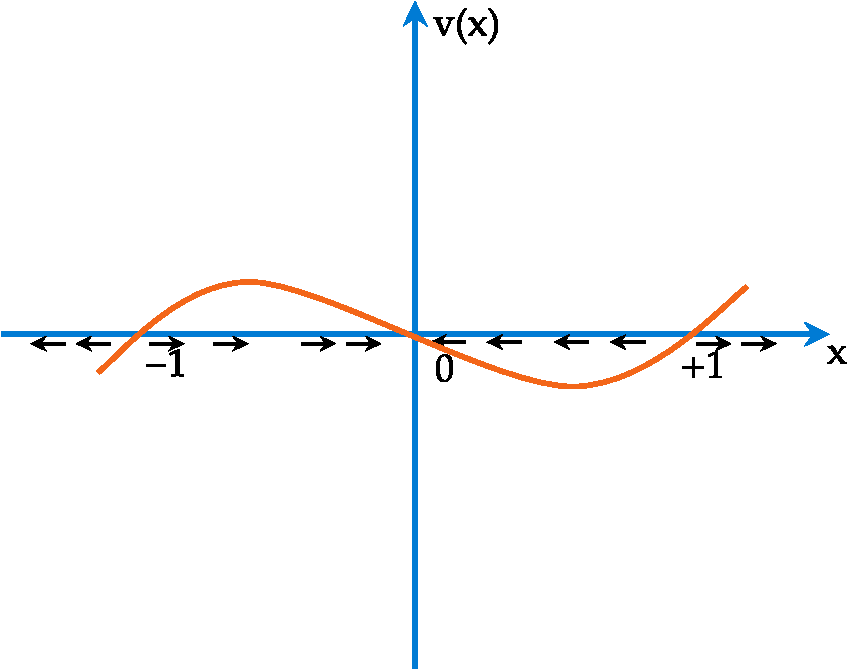
\includegraphics[height=5cm,width=5cm]{diagram-20220214-crop}
		\caption{}
		\label{}
	\end{figure}
\end{itemize}
\textbf{ Properties of Fixed Points}
\begin{itemize}
	\item  The set of zeros of the function $v(x)$ are called the fixed points of the system. The fixed points divide the phase space into several regions.
	\item $x_{k}$ is \textbf{a stable fixed point or sink} if the flow is directed towards the fixed point, otherwise $x_{k}$ is an \textbf{unstable fixed point or repellor.} In the above example obviously $x_{k}=0$ is a stable fixed point where as $x_{k}=\pm 1$ are unstable. It is easy to see that the system evolves towards stable fixed point and away from an unstable fixed point. That is, if $x_{0}$ is a fixed point then define
	$$
	\lambda=\left.\frac{d v}{d x}\right|_{x_{0}}
	$$
	If $\lambda<0$ the fixed point is stable otherwise it is unstable. $\lambda$ is called the characteristic value or some times called Lyapunov exponent.
	\item A fixed point may be both stable and unstable, ie., the neighbouring states approach the fixed point on one side but leave from the other side. We call this a \textbf{saddle point}. This property leads to the so called structural instability, that is even a small perturbation some time can change the nature of fixed point. For example analyse the system with $v(x)=x^{2}$.
	\item The system can not cross a fixed point, by definition. The motion is therefore bounded by the fixed point or fixed points. A system which starts out in the open interval between fixed points remains there for arbitrarily long periods of time. These intervals are therefore called invariant sets. In the example- 4 above the invariant sets are $(-\infty,-1) ;(-1,0) ;(0,1) ;(1, \infty)$
\end{itemize}
Often the motion may be terminating. The terminating motion happens when at some time $t$ the solution of the differential equation is undefined.




\section{Potential energy and equilibrium}
In order to understand the general theory of oscillations, it is essential to know about the potential energl at the equilibrium configuration. Let us consider a conservative system in which the potential energy is: function of position only. Let the system be specified by $n$ generalized coordinates $q_{1}, q_{2}, \ldots, q_{n}$, not involve, time explicitly. For such a system, the potential energy is given by
$$
V=V\left(q_{1}, q_{2}, \ldots, q_{n}\right)
$$
and the generalized forces are given by
$G_{k}=-\frac{\partial V}{\partial q_{k}}$ where $k=1,2, \ldots ., n$\\
The system is said to be in equilibrium, if the generalized forces acting on the system are equal to zero: i.e.,
$$
G_{k}=-\left[\frac{\partial V}{\partial q_{k}}\right]_{0}=0
$$


\section{Stable,Unstable and Neutral equilibrium}
\subsubsection{Stable equilibrium}
A system is said to be in stable equilibrium, if a small displacement of the system from the rest position (by giving a little energy to it) results in a small bounded motion about the equilibrium position.
\subsubsection{Unstable equilibrium}
Small displacement of the system from the equilibrium position results in an unbounded motion, it is in an unstable equilibrium.
\subsubsection{Neutral equilibrium}
Further, if the system on displacement has no tendency to move about or away the equilibrium position, it is said to be in neutral equilibrium.\\
\begin{minipage}{0.5\textwidth}
	\begin{figure}[H]
		\centering
		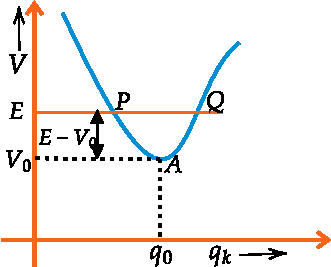
\includegraphics[height=4cm,width=5cm]{stable}
		\caption{}
		\label{fig1}
	\end{figure}
\end{minipage}
\begin{minipage}{0.5\textwidth}
	\begin{figure}[H]
		\centering
		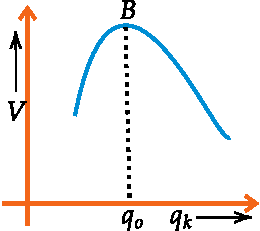
\includegraphics[height=3cm,width=5cm]{unstable}
		\caption{}
		\label{fig2}
	\end{figure}
\end{minipage}
A graph drawn between the potential energy of the system and a particular coordinate $q_{k}$ is called potential energy curve and  The positions $A$ and $B$, where the generalized force $F=-\partial V / \partial q$ vanishes, are the positions of equilibrium; potential energy $V$ is minimum (say $V_{0}$ ) at $A$ [fig.\ref{fig1}] and maximum at $B$ [fig.\ref{fig2} ]. Position $A$ corresponds to the stable equilibrium, because if the system is displaced from $A$ to $Q$ by giving energy $\left(E-V_{0}\right)$ and left to itself, the system tries to come in the position of minimum potential energy. Consequently the potential energy will change to kinetic energy and at $A$ the energy $\left(E-V_{0}\right)$ will be purely in the kinetic form because of the conservation law. This will change again to potential form, when the system moves towards the position $P$ and hence a bounded motion ensues about the equilibrium position $A$. Obviously the position $B$ of the maximum potential energy represents the unstable equilibrium because any energy given to the system at this position will result more and more kinetic energy when the system moves either left or right to it. In this case, the system moves away from the equilibrium position. In case of neutral equilibrium, the potential energy is independent of the coordinate and equilibrium. occurs at any arbitrary value of that coordinate.



\section{How to draw a phase curve:}
Step 1: Draw a curve of potential $U(x)\quad V_{S} \quad x$, where $U(x)$ as vertical axis and $x$ as horizontal axis.\\
Step 2: Just below of potential $U(x)$ vs $x$ curve, draw momentum $P(x)$ as vertical axis and $x$ as horizontal axis.\\
Step 3: For different values of constant energy in $U(x) V s x$ draw the trend of $P(x)$ vs $x$ in all classical allowed region.\\
Step 4: Use sign convention as mention above.




\subsection{ Simple Pendulum}
In this example, because the Hamiltonian is constant and equal to the energy of the system, the easiest way to generate a phase plot is to derive the Hamiltonian in terms of $\boldsymbol{p}$ and $\boldsymbol{q}$. The Hamiltonian of the simple pendulum illustrated in Figure 1, consisting of a mass $m$ suspended by a massless string of length $l$ is given by:
$$
H(\theta, p)=T+V=\frac{p^{2}}{2 m l^{2}}-m g l \cos \theta
$$
In this particular case, it's obvious that $\theta=q$, the generalized coordinate and the Hamiltonian is timeindependent and is equal to the total energy of the pendulum system.\\
Figure 2 is the phase-space representation of the motion of the pendulum for four different values of the Hamiltonian or energy of the system.\\
\par The innermost (green) curve or trajectory represents the motion of the pendulum for the lowest of the four energy levels. The pendulum has sufficient energy to swing through an angle of approximately $\pm \frac{\pi}{2}$ and obviously has the lowest maximum value of momentum. As time advances, the phase point representing the instantaneous state of the pendulum system repeatedly traces out the green trajectory, one period represented by a single orbit.
The blue trajectory represents the motion of the pendulum with slightly higher energy than the green trajectory as demonstrated by the higher maximum value for the momentum and $\theta$.
The purple trajectory represents a higher energy than the blue or green and shows the swing angle $\theta$ approaching $\pm \pi$, the maximum swing angle while still retaining 'back and forth' motion.
The orange, outermost trajectory represents the highest of the four energy levels and clearly demonstrates that the pendulum is now rotating continuously in one direction (no longer exhibiting 'back and forth' motion) by virtue of the open trajectory. An obvious implication of the open trajectory is that the system's momentum never falls to zero and continues in the same direction without limit.\\
\begin{figure}[H]
	\centering
	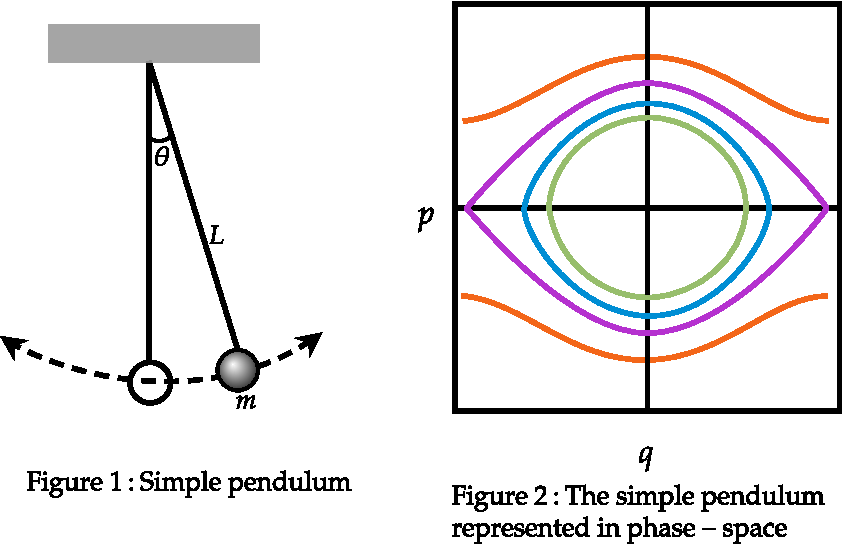
\includegraphics[height=6cm,width=10cm]{diagram-20220215(7)-crop}
	\caption{}
	\label{}
\end{figure}
The phase-space trajectory that represents the motion of the pendulum at the limit where the motion changes from 'back and forth' to continuous rotation is called the separatrix. The purple trajectory in figure 2 is very close in energy to the separatrix and is extremely close to it in shape.\\
\begin{note}
	$\text { Driven, damped SHO at resonance. }$\\
	\begin{figure}[H]
		\centering
		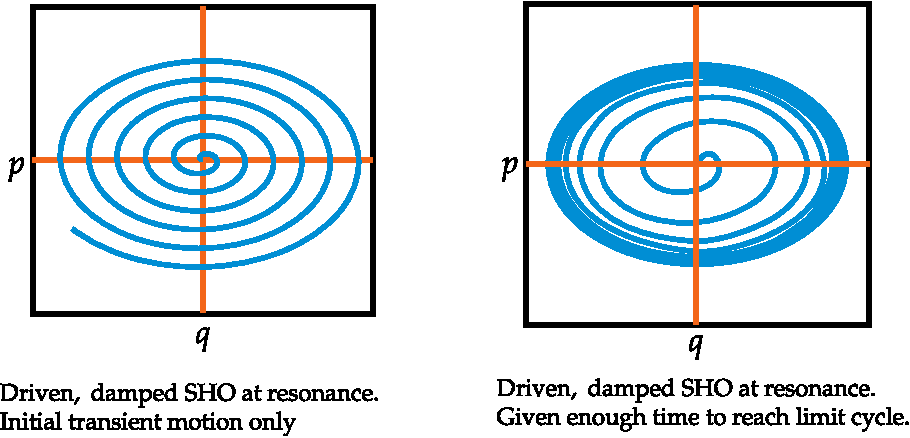
\includegraphics[height=6cm,width=10cm]{diagram-20220215(11)-crop}
		\caption{}
		\label{}
	\end{figure}
\end{note}



\begin{example}
	If potential in one dimension is given by $V(x)=-\frac{x^{2}}{2}+\frac{x^{4}}{4}$ then plot the phase curve ie curve between momentum $p_{x}$ as function of $x$ for all possible range of energy $E$.
\end{example}
\begin{answer}
	To plot phase curve first one should plot potential $(V$ vs $x)$, then on the same axis one should plot momentum with common $x$ axis.
	
	We can check how momentum is changing with position keeping in mind how potential is changing with position.
	
	One will plot the phase curve by assuming that if the potential is increasing, then kinetic energy will be decreasing and if the potential is decreasing, then kinetic energy will be increasing because total energy will always remain constant. One should plot the phase curve for different range of energy.
	For example in the given potential, there are three range of energy.\\
	For example in the given potential, there are three range of energy.\\ 
	\textbf{Case 1:}  If $-\frac{1}{4}<E<0$ the particle has motion about stable equilibrium point $x=1,-1$ the motion is bounded.\\
	\textbf{Case 2:} If $0<E<\infty$ the particle has motion about unstable equilibrium point $x=0$ the motion is bounded.
	\textbf{Case 3:} At $E=0$ the particle can be landed exactly at unstable equilibrium point which is nature of transition from case 1 to case 2 .\\
	\textcolor{red}{figure}
	\begin{figure}[H]
		\centering
		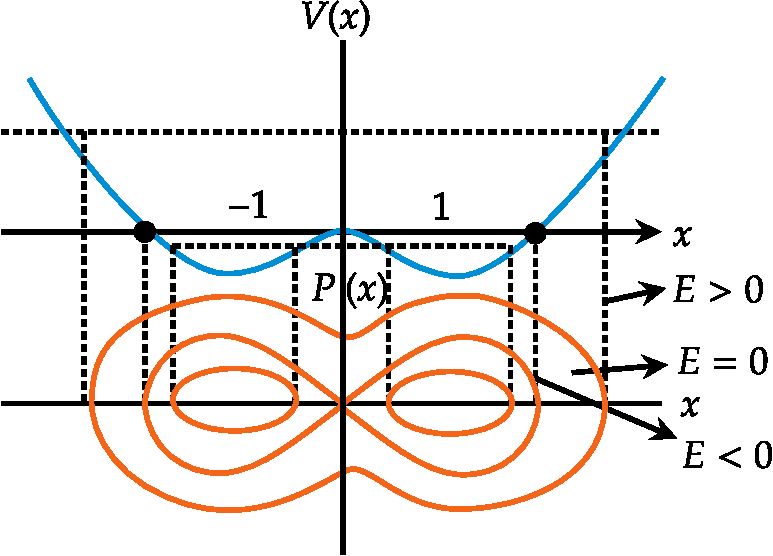
\includegraphics[height=5cm,width=7cm]{diagram-20220222-crop}
	\end{figure}
\end{answer}
\begin{example}
	If potential in one dimension is given by $V(x)=-k x^{2}$ then plot the phase curve i.e. curve between momentum $p_{x}$ as function of $x$ for all possible range of energy $E$.
\end{example}
\begin{answer}
	To plot phase curve first one should plot potential $(V$ vs $x)$, then on the same axis one should plot momentum with common $x$ axis .
	
	We can check how momentum is changing with position keeping in mind how potential is changing for a given value of energy. For given value of potential the phase curve is hyperbolic as shown in equation $E=\frac{p_{x}^{2}}{2 m}-k x^{2} \Rightarrow \frac{p_{x}^{2}}{2 m E}-\frac{x^{2}}{E / k}=1$\\
	One will plot the phase curve by assuming that if the potential is increasing, then kinetic energy will be decreasing and if potential is decreasing then kinetic energy will be increasing, because total energy will always remain constant. One should plot the phase curve for different range of energy. For example in this potential there are three range of energy\\
	\textbf{Case 1:} $E<0$, the particle will come from $-\infty .$ As it is approaches the potential its kinetic energy as well as momentum decreases finally became zero at turning point $A$ and turn back towards $-\infty$ with increasing kinetic energy and momentum.\\
	Same trend will also follow when particle approaching the potential from $x=\infty$, for turning point $A^{\prime}$.\\
	\textbf{Case 2:} $E>0$, the particle will come from $x=-\infty$. As it approaches the potential. its kinetic energy as well as momentum decreases till $x=0$. As it crosses $x=0$ and move towards $x=\infty$, again kinetic energy as well as momentum increases and same trend will be followed, when particle approaches the potential to $x=\infty$.\\
	\textbf{Case 3:} $E=0$, the particle can reach at $x=0$, which is unstable equilibrium point and the phase curve will also be separated between $E<0$ and $E>0$, identified as separatix. $E=\frac{p_{x}^{2}}{2 m}-k x^{2}$ for $E=0 \Rightarrow p_{x} \propto \pm x$ which is straight line.\\
	\begin{figure}[H]
		\centering
		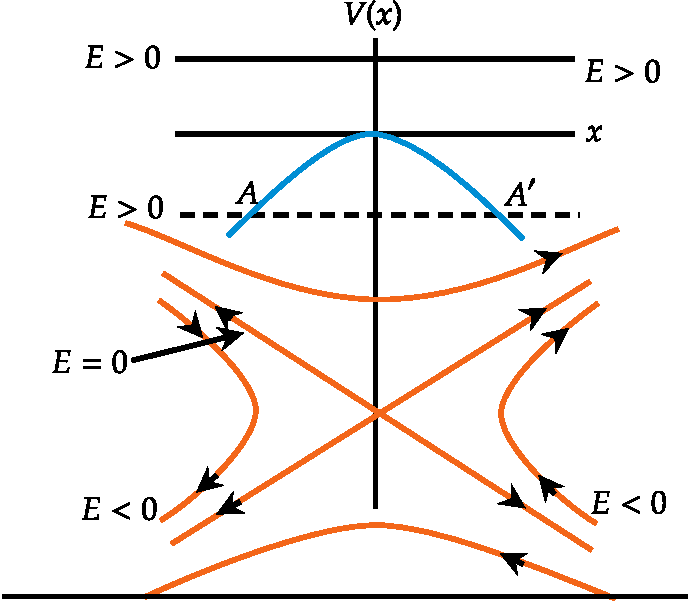
\includegraphics[height=5cm,width=7cm]{diagram-20220222(1)-crop}
	\end{figure}
\end{answer}
\begin{example}
	The energy of simple pendulum is given by $E=\frac{p_{\theta}^{2}}{2 m a^{2}}-m g a \cos \theta$, where $p_{\theta}$ angular momentum and $-m g a \cos \theta$ is potential energy.
\end{example}
\begin{answer}
	One will plot the phase curve by assuming that if the potential energy is increasing, then kinetic energy will be decreasing and if the potential energy is decreasing then kinetic energy will be increasing, because total energy will always remain constant. One should plot the phase curve for different range of energy. For example in this potential there are three range of energy.
	The stable equilibrium point is $\theta=0$. $\theta=-\pi$ and $\theta=\pi$ are unstable equilibrium points.\\
	\textbf{Case 1:}$\text { For energy }-m g a<E<m g a$  particle is bounded about stable equilibrium point .so phase curve is periodic.\\
	\textbf{Case 2:} For energy $E>m g a$ motion will become unbounded and phase curve will be a periodic. Liberation will take place.\\
	\textbf{Case 3:} For energy $E=m g a$ particle will reach at unstable equilibrium point it also separate two type of motion (mention in case 1 and case 2 ) identified as separatix.
	\begin{figure}[H]
		\centering
		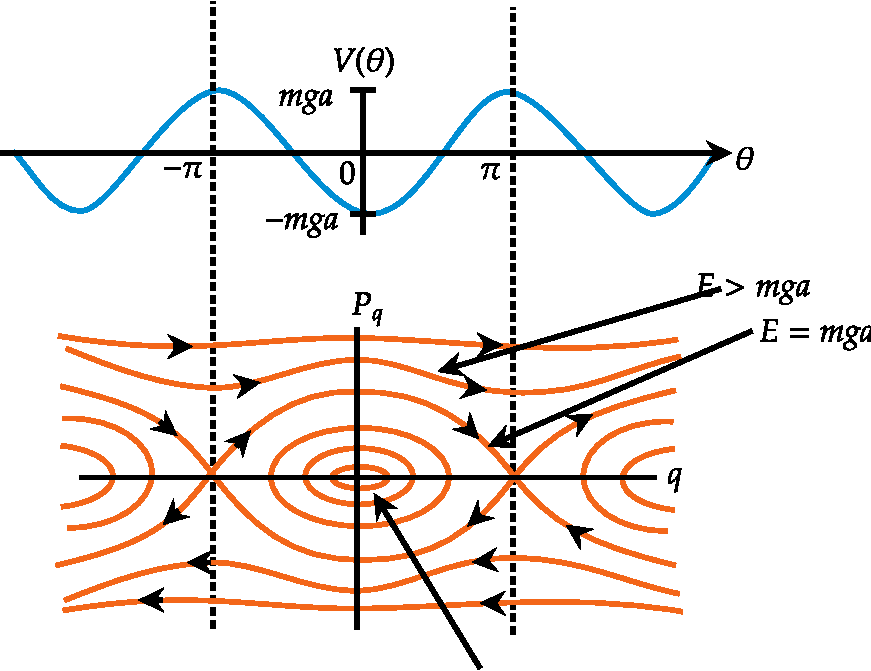
\includegraphics[height=5cm,width=7cm]{diagram-20220222(2)-crop}
	\end{figure}
\end{answer}
\begin{example}
	Phase curves for the Kepler effective potential $U(x)=-x^{-1}+\frac{1}{2}x^{-2}$
\end{example}
\begin{answer}
	\begin{figure}[H]
		\centering
		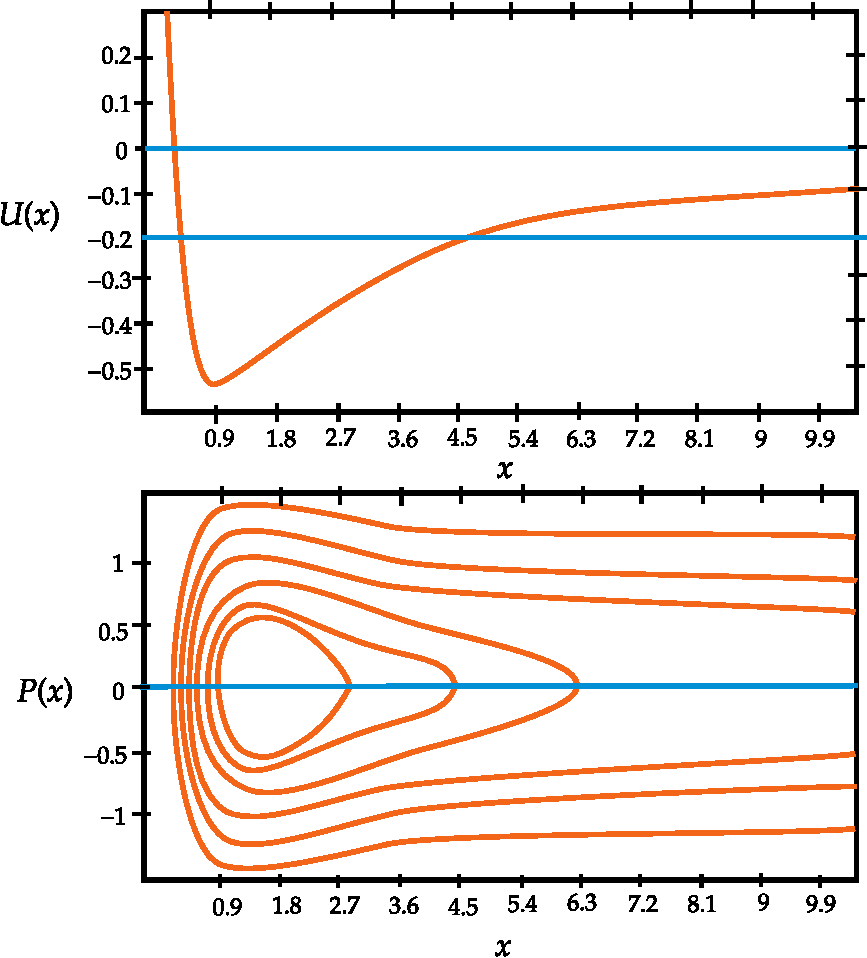
\includegraphics[height=5cm,width=7cm]{diagram-20220225(2)-crop}
	\end{figure}
\end{answer}
\begin{example}
	Phase space trajecteries for double well potential
\end{example}
\begin{answer}
	\begin{figure}[H]
		\centering
		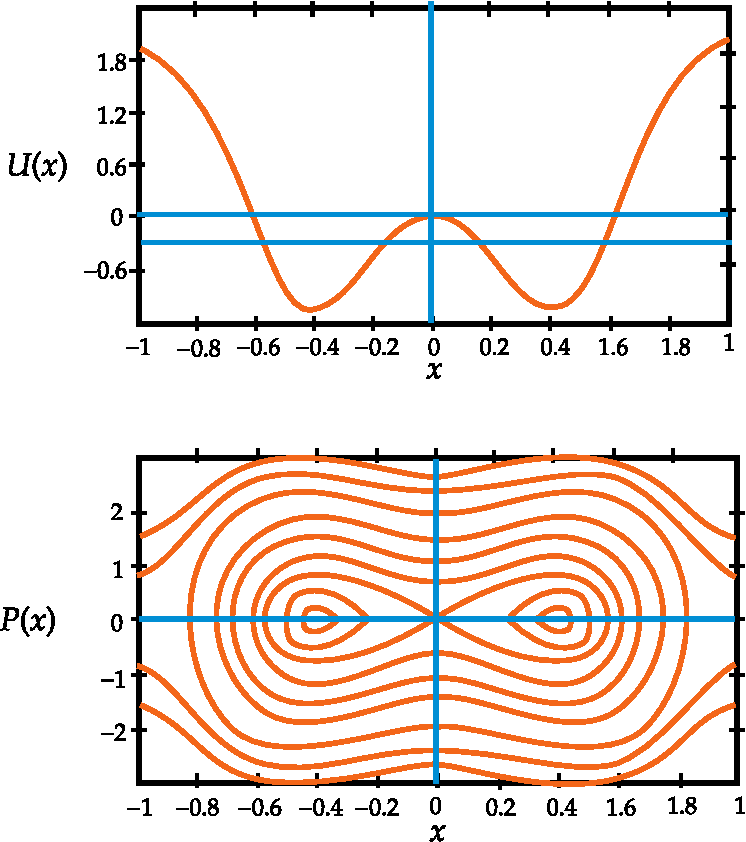
\includegraphics[height=5cm,width=7cm]{phase 2}
	\end{figure}	
\end{answer}
\begin{example}
	Phase curves for the potential $U(x)=-\sech^2(x)$
\end{example}
\begin{answer}
	\begin{figure}[H]
		\centering
		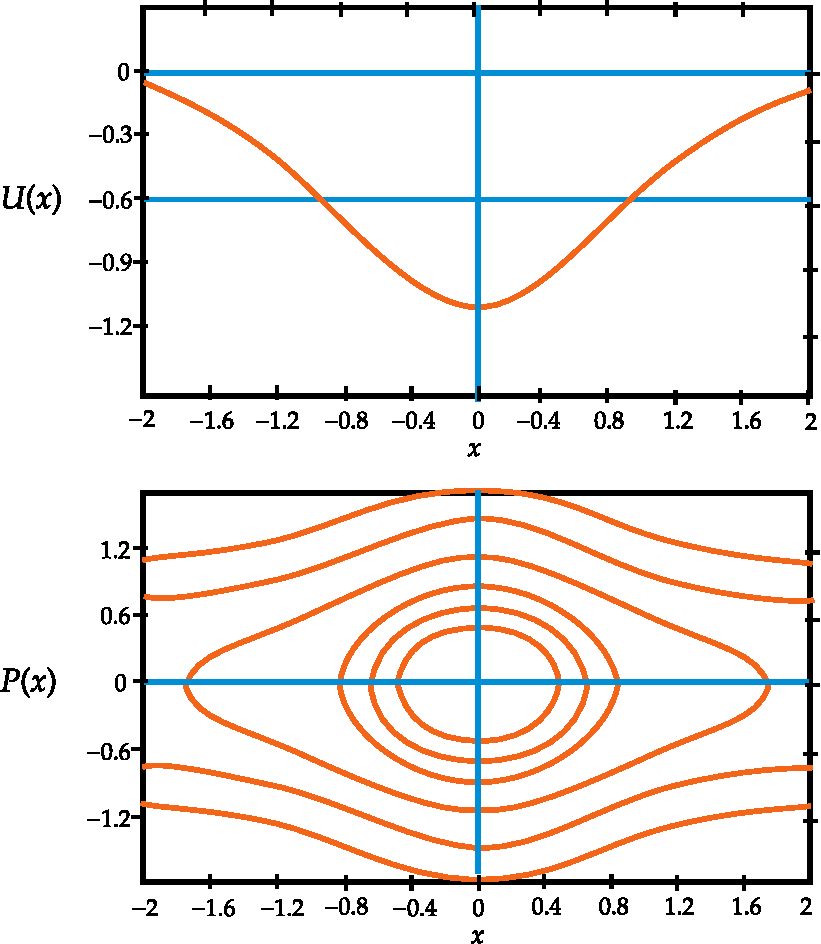
\includegraphics[height=5cm,width=7cm]{phase 3}
	\end{figure}	
\end{answer}




\newpage
\begin{abox}
	Practice set 1 
\end{abox}
\begin{enumerate}
	\item The trajectory on the $z p_{z}$ - plane (phase-space trajectory) of a ball bouncing perfectly elastically off a hard surface at $z=0$ is given by approximately by (neglect friction):
	{\exyear{NET JUNE 2011}}
	\begin{tasks}(2)
		\task[\textbf{A.}]\begin{figure}[H]
			\centering
			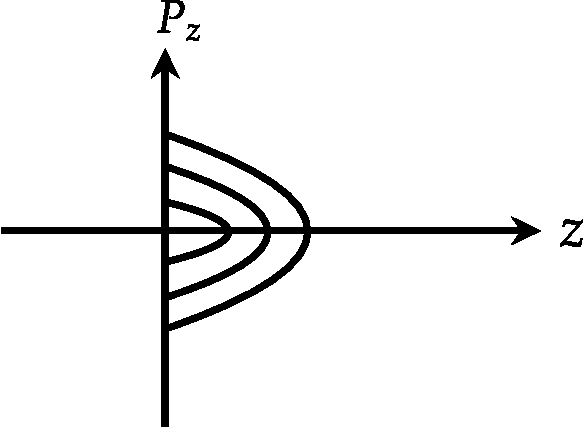
\includegraphics[height=3cm,width=5cm]{diagram-20210926(3)-crop}
		\end{figure}
		\task[\textbf{B.}]\begin{figure}[H]
			\centering
			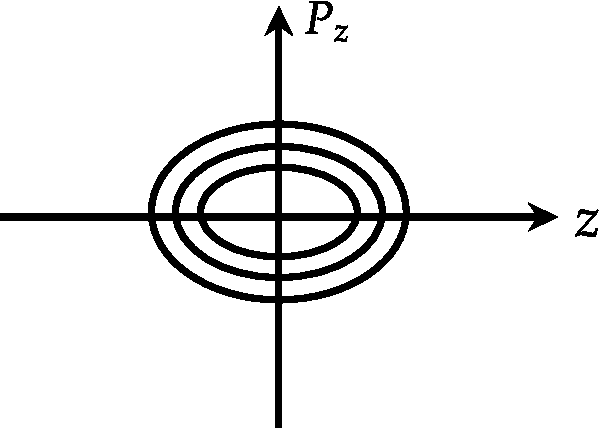
\includegraphics[height=3cm,width=5cm]{diagram-20210926(4)-crop}
		\end{figure}
		\task[\textbf{C.}]\begin{figure}[H]
			\centering
			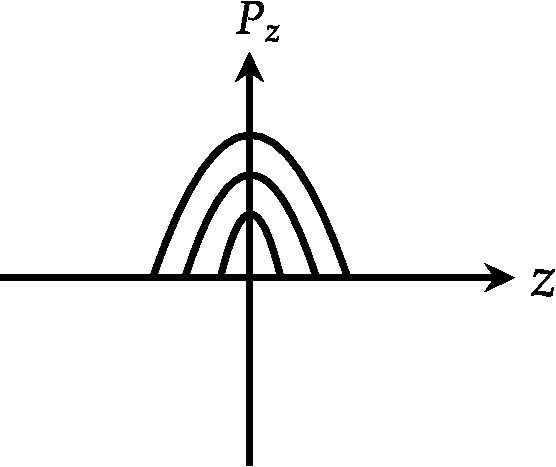
\includegraphics[height=3cm,width=5cm]{diagram-20210926(5)-crop}
		\end{figure}
		\task[\textbf{D.}]\begin{figure}[H]
			\centering
			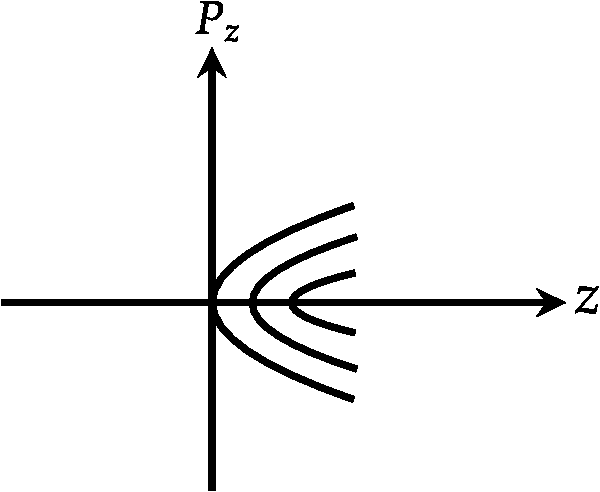
\includegraphics[height=3cm,width=5cm]{diagram-20210926(6)-crop}
		\end{figure}
	\end{tasks}
	\item The bob of a simple pendulum, which undergoes small oscillations, is immersed in water. Which of the following figures best represents the phase space diagram for the pendulum?
	{\exyear{NET JUNE 2012}}
	\begin{tasks}(2)
		\task[\textbf{A.}]\begin{figure}[H]
			\centering
			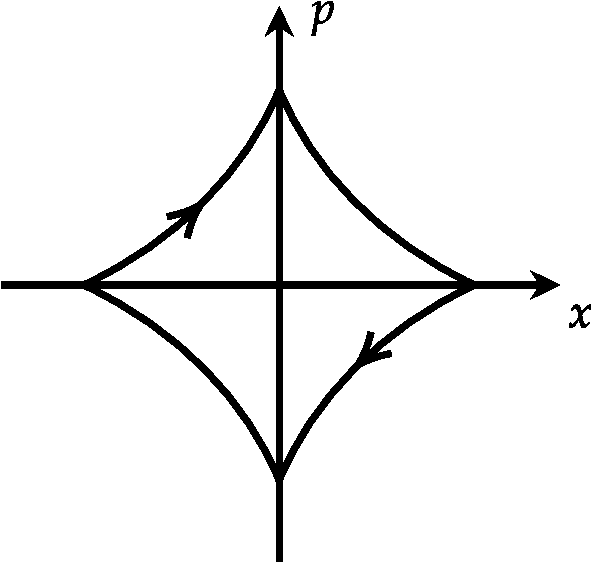
\includegraphics[height=3cm,width=5cm]{diagram-20210926(7)-crop}
		\end{figure}
		\task[\textbf{B.}]\begin{figure}[H]
			\centering
			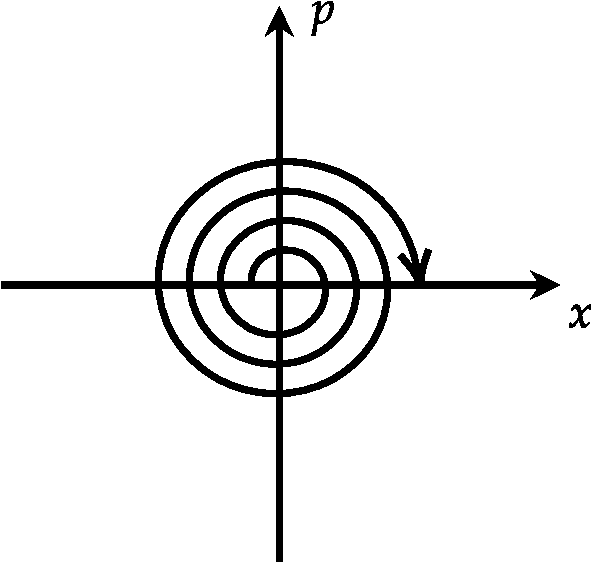
\includegraphics[height=3cm,width=5cm]{diagram-20210926(8)-crop}
		\end{figure}
		\task[\textbf{C.}]\begin{figure}[H]
			\centering
			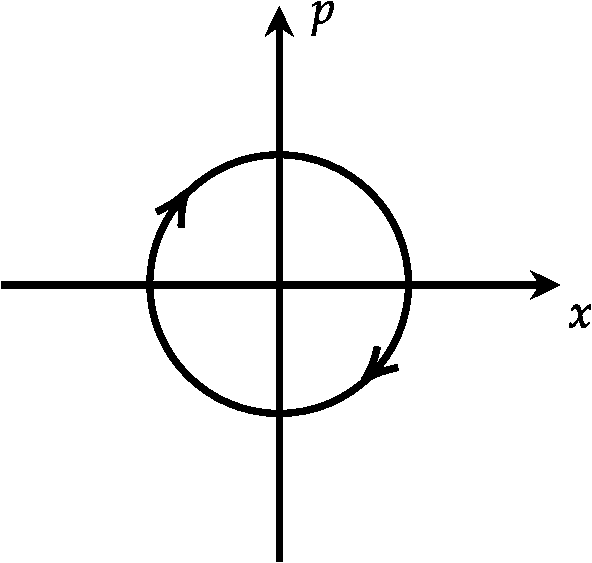
\includegraphics[height=3cm,width=5cm]{diagram-20210926(9)-crop}
		\end{figure}
		\task[\textbf{D.}]\begin{figure}[H]
			\centering
			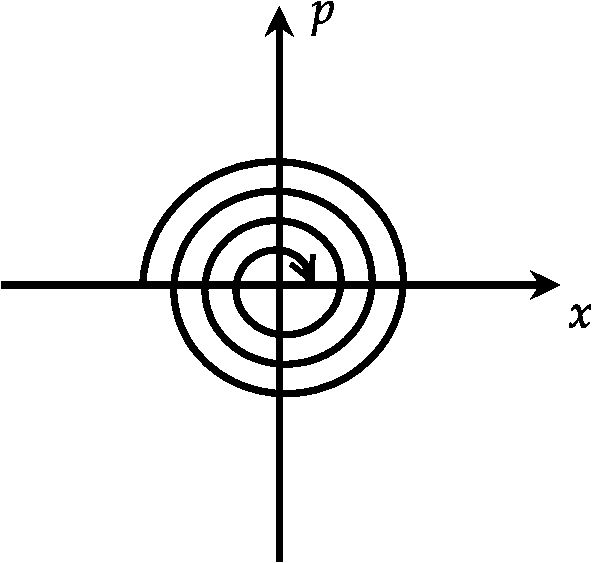
\includegraphics[height=3cm,width=5cm]{diagram-20210926(10)-crop}
		\end{figure}
	\end{tasks}
	\item Which of the following set of phase-space trajectories is not possible for a particle obeying Hamilton's equations of motion?
	{\exyear{NET DEC 2012}}
	\begin{tasks}(2)
		\task[\textbf{A.}]\begin{figure}[H]
			\centering
			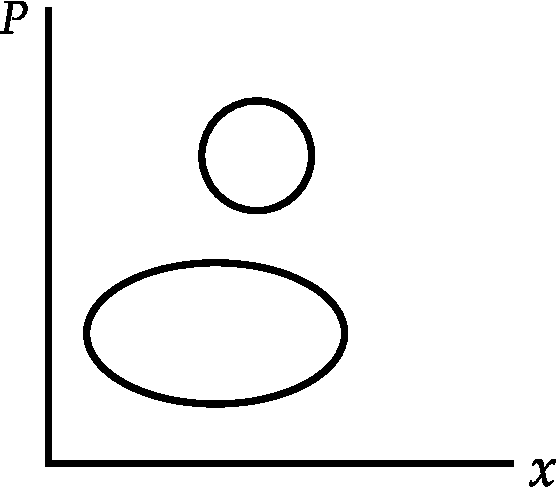
\includegraphics[height=3cm,width=5cm]{diagram-20210926(13)-crop}
		\end{figure}
		\task[\textbf{B.}]\begin{figure}[H]
			\centering
			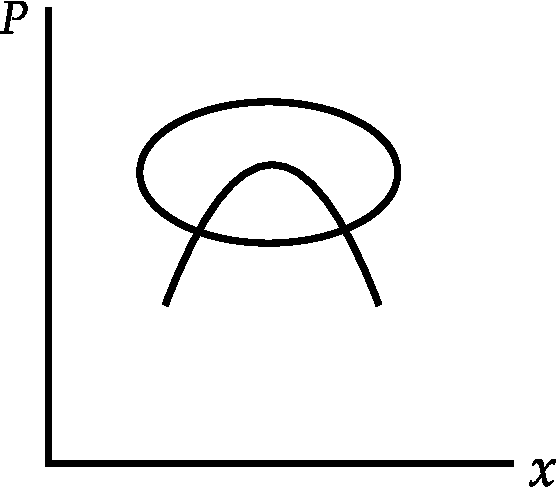
\includegraphics[height=3cm,width=5cm]{diagram-20210926(14)-crop}
		\end{figure}
		\task[\textbf{C.}]\begin{figure}[H]
			\centering
			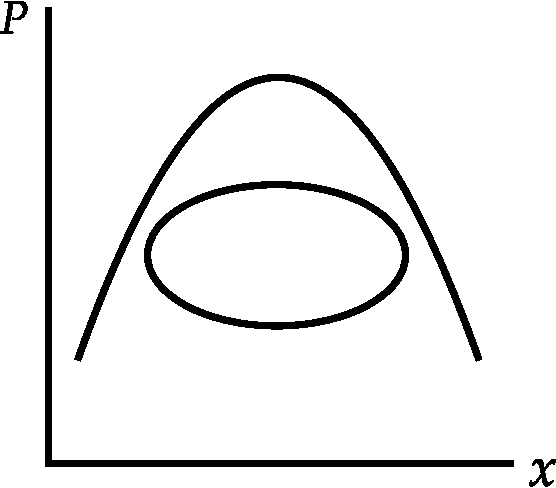
\includegraphics[height=3cm,width=5cm]{diagram-20210926(15)-crop}
		\end{figure}
		\task[\textbf{D.}]\begin{figure}[H]
			\centering
			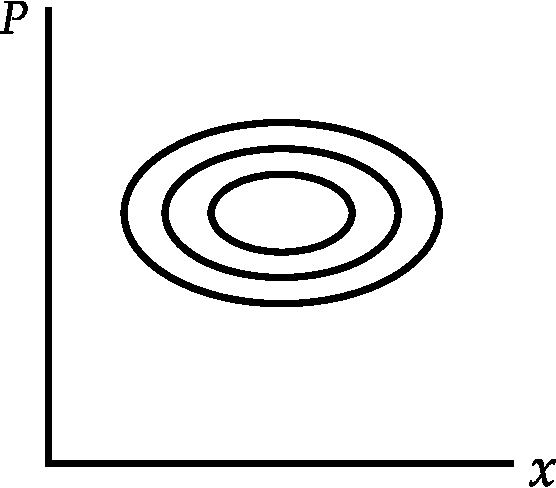
\includegraphics[height=3cm,width=5cm]{diagram-20210926(16)-crop}
		\end{figure}
	\end{tasks}
	\item The Hamiltonian of a classical particle moving in one dimension is $H=\frac{p^{2}}{2 m}+\alpha q^{4}$ where $\alpha$ is a positive constant and $p$ and $q$ are its momentum and position respectively. Given that its total energy $E \leq E_{0}$ the available volume of phase space depends on $E_{0}$ as
	{\exyear{NET DEC 2014}}
	\begin{tasks}(2)
		\task[\textbf{A.}] $E_{0}^{3 / 4}$
		\task[\textbf{B.}]$E_{0}$
		\task[\textbf{C.}]$\sqrt{E_{0}}$
		\task[\textbf{D.}]is independent of $E_{0}$
	\end{tasks}
	\item Which of the following figures is a schematic representation of the phase space trajectories (i.e., contours of constant energy) of a particle moving in a one-dimensional potential $V(x)=\frac{-1}{2} x^{2}+\frac{1}{4} x^{4}$
	{\exyear{NET JUNE 2015}}
	\begin{tasks}(2)
		\task[\textbf{A.}]\begin{figure}[H]
			\centering
			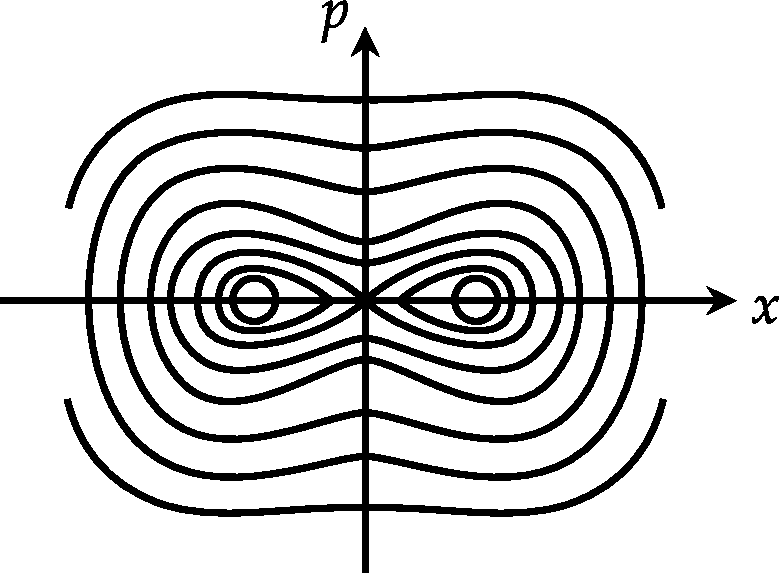
\includegraphics[height=3cm,width=5cm]{diagram-20210926(24)-crop}
		\end{figure}
		\task[\textbf{B.}]\begin{figure}[H]
			\centering
			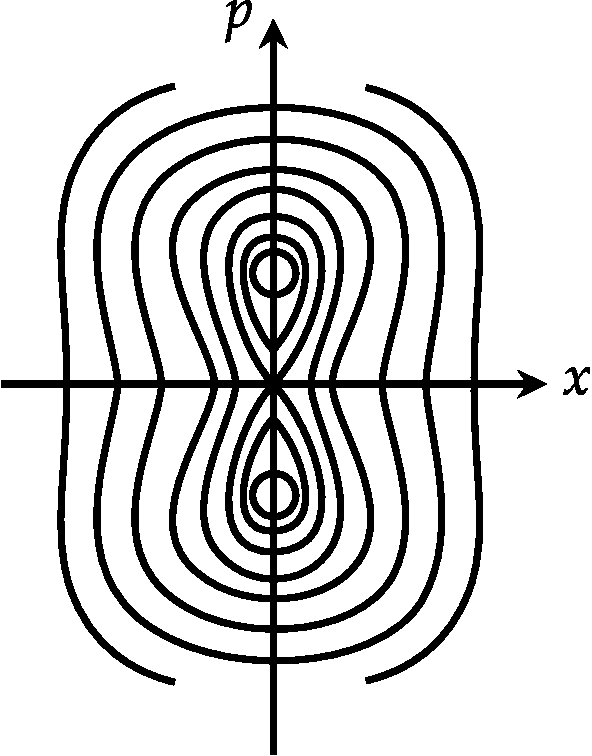
\includegraphics[height=3cm,width=5cm]{diagram-20210926(25)-crop}
		\end{figure}
		\task[\textbf{C.}]\begin{figure}[H]
			\centering
			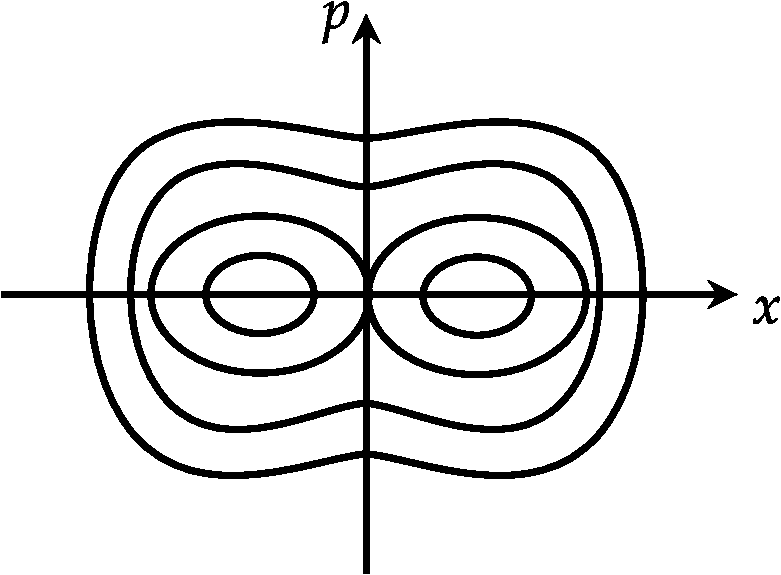
\includegraphics[height=3cm,width=5cm]{diagram-20210926(26)-crop}
		\end{figure}
		\task[\textbf{D.}]\begin{figure}[H]
			\centering
			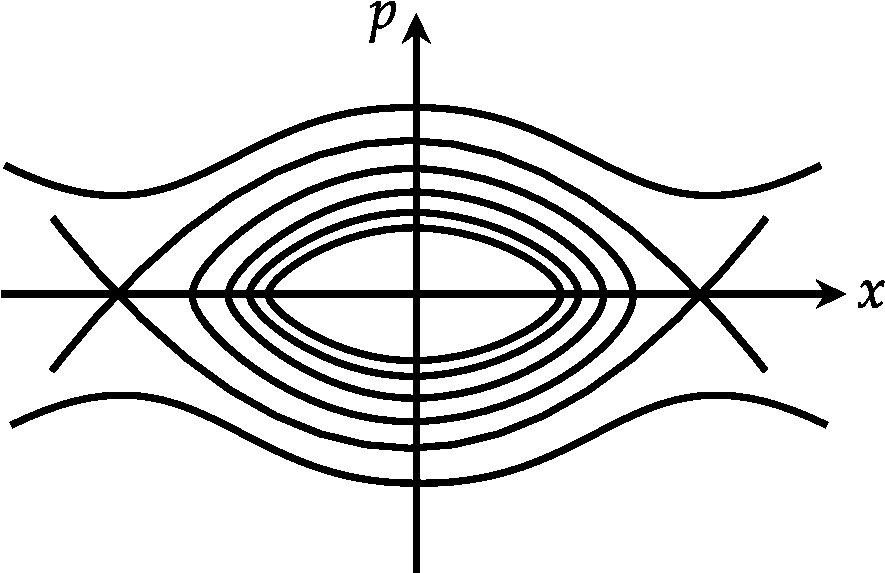
\includegraphics[height=3cm,width=5cm]{diagram-20210926(27)-crop}
		\end{figure}
	\end{tasks}
	\item A particle moves in one dimension in a potential $V(x)=-k^{2} x^{4}+\omega^{2} x^{2}$ where $k$ and $\omega$ are constants. Which of the following curves best describes the trajectories of this system in phase space?
	{\exyear{NET DEC 2017}}
	\begin{tasks}(2)
		\task[\textbf{A.}]\begin{figure}[H]
			\centering
			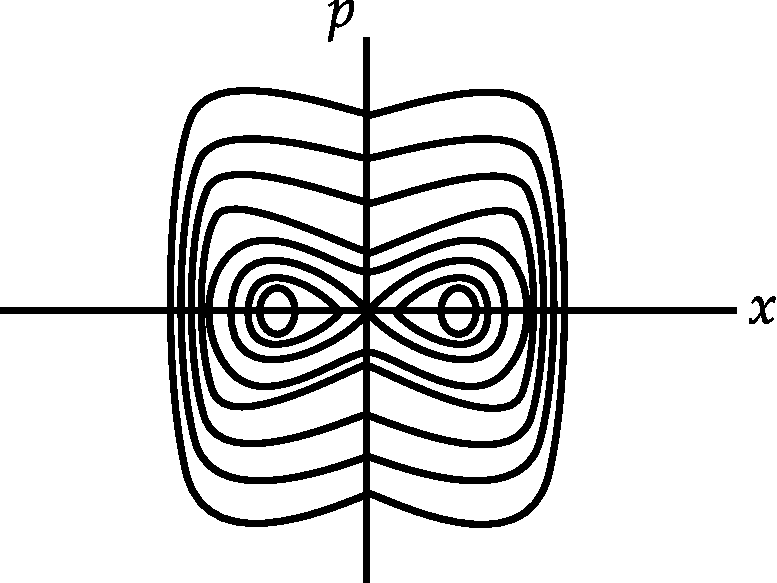
\includegraphics[height=3cm,width=5cm]{diagram-20210926(42)-crop}
		\end{figure}
		\task[\textbf{B.}]\begin{figure}[H]
			\centering
			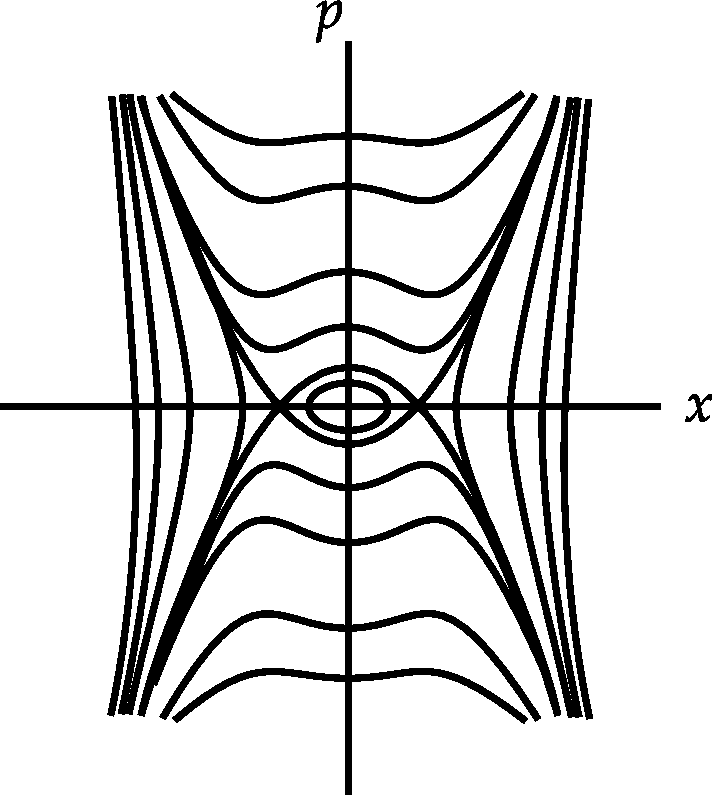
\includegraphics[height=3cm,width=5cm]{diagram-20210926(43)-crop}
		\end{figure}
		\task[\textbf{C.}]\begin{figure}[H]
			\centering
			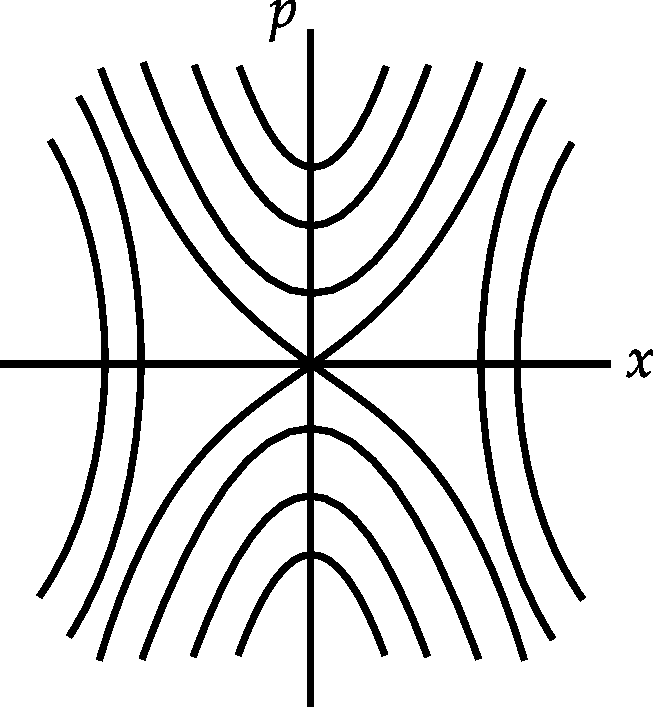
\includegraphics[height=3cm,width=5cm]{diagram-20210926(44)-crop}
		\end{figure}
		\task[\textbf{D.}]\begin{figure}[H]
			\centering
			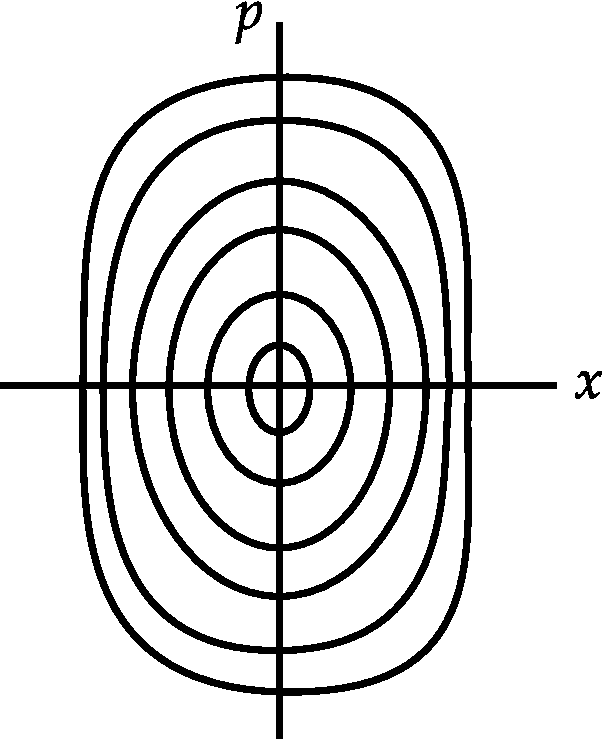
\includegraphics[height=3cm,width=5cm]{diagram-20210926(45)-crop}
		\end{figure}
	\end{tasks}
\end{enumerate}
\colorlet{ocre1}{ocre!70!}
\colorlet{ocrel}{ocre!30!}
\setlength\arrayrulewidth{1pt}
\begin{table}[H]
	\centering
	\arrayrulecolor{ocre}
	
	\begin{tabular}{|p{1.5cm}|p{1.5cm}||p{1.5cm}|p{1.5cm}|}
		\hline
		\multicolumn{4}{|c|}{\textbf{Answer key}}\\\hline\hline
		\rowcolor{ocrel}Q.No.&Answer&Q.No.&Answer\\\hline
		1&\textbf{a}&2&\textbf{d}\\\hline
		3&\textbf{b}&4&\textbf{a}\\\hline
		5&\textbf{a}&6&\textbf{c}\\\hline
	\end{tabular}
\end{table}
\newpage
\begin{abox}
	Practice set 2
\end{abox}
\begin{enumerate}
	\item The Hamiltonian of particle of mass $m$ is given by $H=\frac{p^{2}}{2 m}-\frac{\alpha q^{2}}{2}$. Which one of the following figure describes the motion of the particle in phase space?
	{\exyear{GATE 2014}}
	
	\begin{tasks}(2)
		\task[\textbf{A.}]\begin{figure}[H]
			\centering
			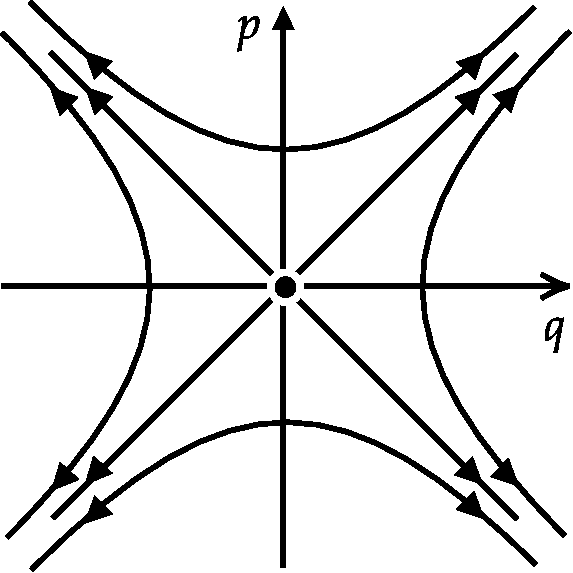
\includegraphics[height=4cm,width=5cm]{diagram-20210915(5)-crop}
		\end{figure}
		\task[\textbf{B.}]\begin{figure}[H]
			\centering
			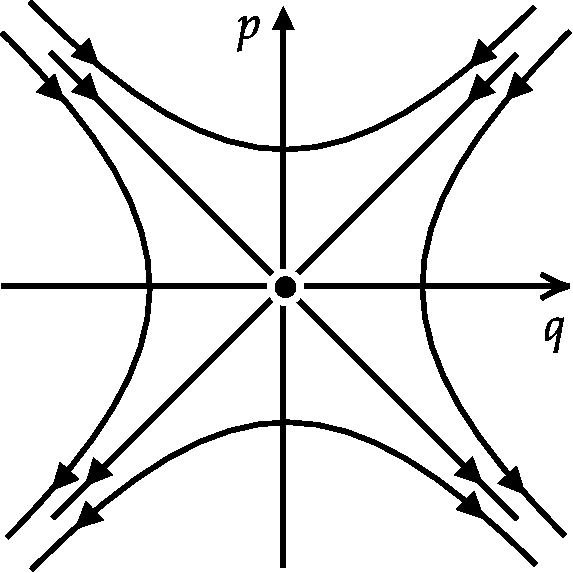
\includegraphics[height=4cm,width=5cm]{diagram-20210915(6)-crop}
		\end{figure}
		\task[\textbf{C.}]\begin{figure}[H]
			\centering
			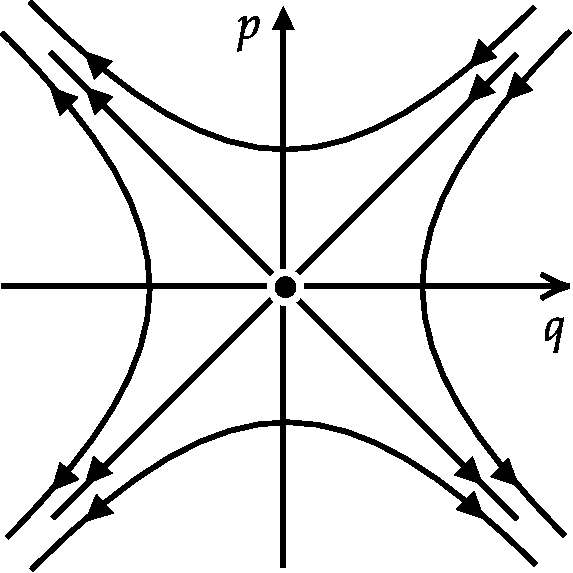
\includegraphics[height=4cm,width=5cm]{diagram-20210915(7)-crop}
		\end{figure}
		\task[\textbf{D.}]\begin{figure}[H]
			\centering
			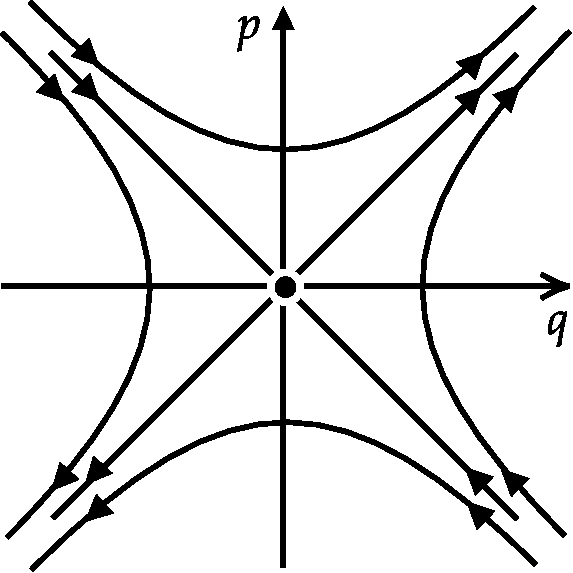
\includegraphics[height=4cm,width=5cm]{diagram-20210915(8)-crop}
		\end{figure}
	\end{tasks}
	\item A particle moves in one dimension under a potential $V(x)=\alpha|x|$ with some non-zero total energy. Which one of the following best describes the particle trajectory in the phase space?
	{\exyear{GATE 2018}}
	
	\begin{tasks}(2)
		\task[\textbf{A.}]\begin{figure}[H]
			\centering
			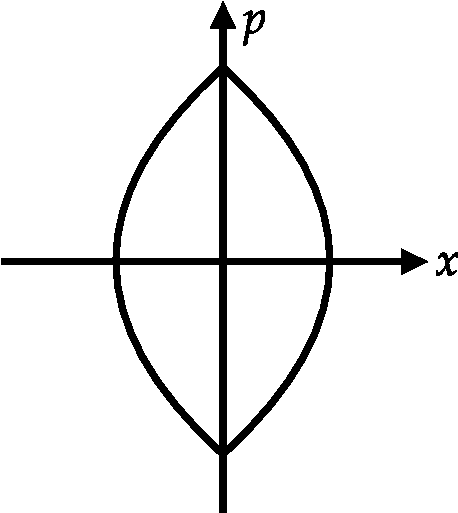
\includegraphics[height=3cm,width=5cm]{diagram-20210915(11)-crop}
			
		\end{figure}
		\task[\textbf{B.}]\begin{figure}[H]
			\centering
			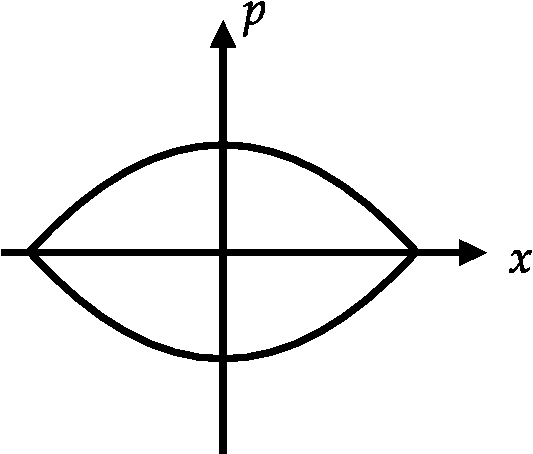
\includegraphics[height=3cm,width=5cm]{diagram-20210915(12)-crop}
		\end{figure}
		\task[\textbf{C.}]\begin{figure}[H]
			\centering
			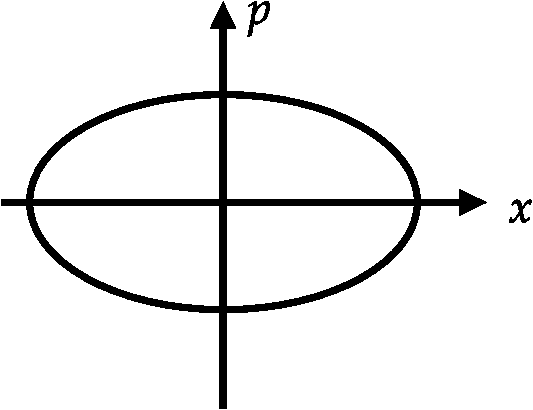
\includegraphics[height=3cm,width=5cm]{diagram-20210915(13)-crop}
		\end{figure}
		\task[\textbf{D.}]\begin{figure}[H]
			\centering
			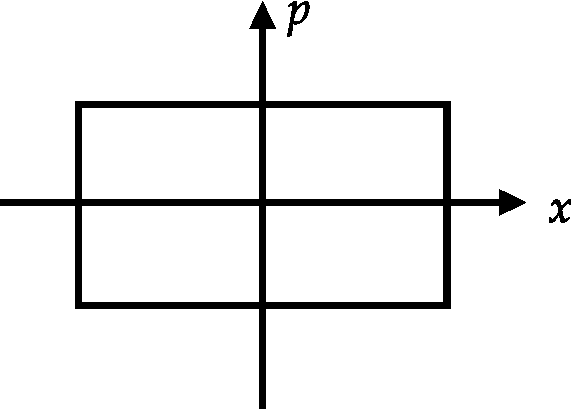
\includegraphics[height=3cm,width=5cm]{diagram-20210915(14)-crop}
		\end{figure}
	\end{tasks}	
	\item A particle moves in one dimension under a potential $V(x)=\alpha|x|$ with some non-zero total energy. Which one of the following best describes the particle trajectory in the phase space?
	{\exyear{GATE 2018}}
	\begin{tasks}(2)
		\task[\textbf{A.}]\begin{figure}[H]
			\centering
			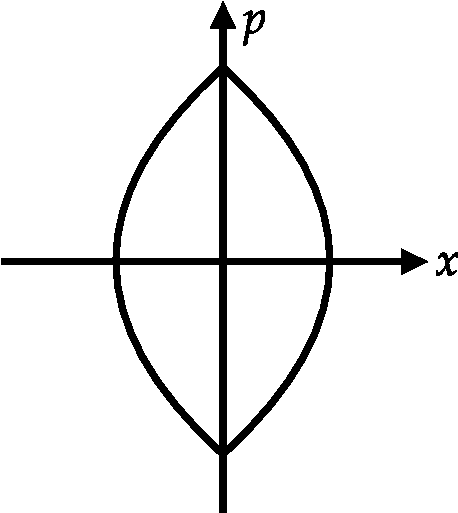
\includegraphics[height=3cm,width=5cm]{diagram-20210915(11)-crop}
			
		\end{figure}
		\task[\textbf{B.}]\begin{figure}[H]
			\centering
			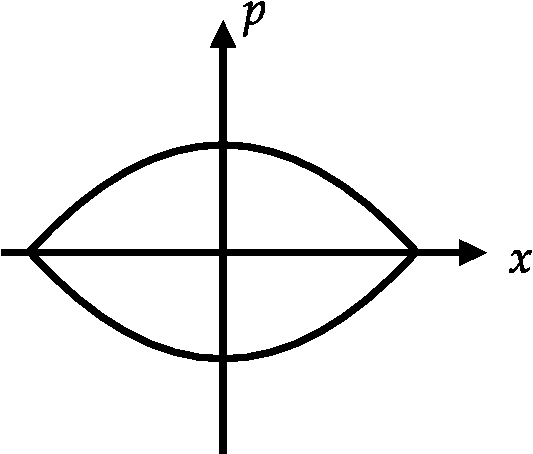
\includegraphics[height=3cm,width=5cm]{diagram-20210915(12)-crop}
		\end{figure}
		\task[\textbf{C.}]\begin{figure}[H]
			\centering
			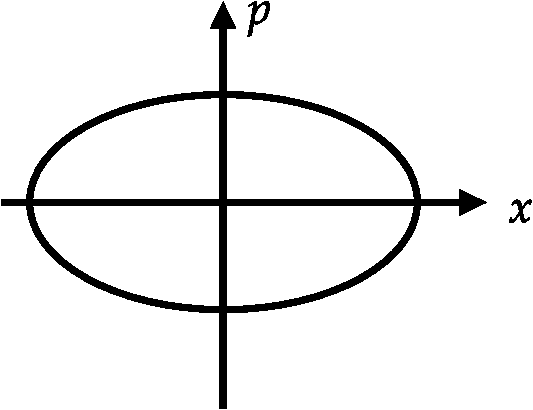
\includegraphics[height=3cm,width=5cm]{diagram-20210915(13)-crop}
		\end{figure}
		\task[\textbf{D.}]\begin{figure}[H]
			\centering
			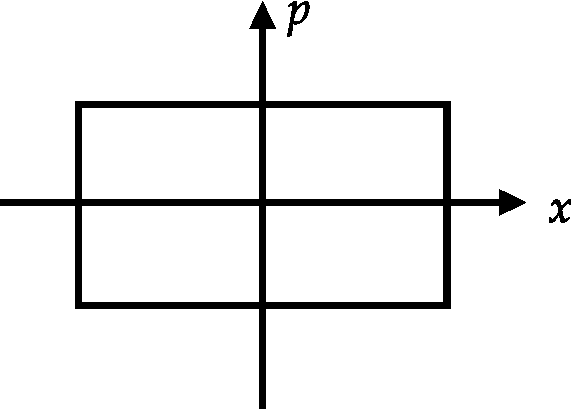
\includegraphics[height=3cm,width=5cm]{diagram-20210915(14)-crop}
		\end{figure}
	\end{tasks}
\end{enumerate}
\colorlet{ocre1}{ocre!70!}
\colorlet{ocrel}{ocre!30!}
\setlength\arrayrulewidth{1pt}
\begin{table}[H]
	\centering
	\arrayrulecolor{ocre}
	
	\begin{tabular}{|p{1.5cm}|p{1.5cm}||p{1.5cm}|p{1.5cm}|}
		\hline
		\multicolumn{4}{|c|}{\textbf{Answer key}}\\\hline\hline
		\rowcolor{ocrel}Q.No.&Answer&Q.No.&Answer\\\hline
		1&\textbf{d}&2&\textbf{a}\\\hline
		3&\textbf{b}&&\\\hline
	\end{tabular}
\end{table}
\newpage
\begin{abox}
	Practise set-3
\end{abox}
\begin{enumerate}[label=\color{ocre}\textbf{\arabic*.}]
	\item  A large mass $\mathrm{M}$ and a small mass ${m}$ hang at the two ends of a string that passes through a smooth tube as shown in fig. The mass $m$ moves around a circular path in a horizontal plane. The length of the string from mass $m$ to the top of the tube is $l$, and $\theta$ is the angle the string makes with the vertical. What should be the frequency $(v)$ of rotation of mass $m$ so that mass	$M$ remains stationary?
	\begin{figure}[H]
		\centering
		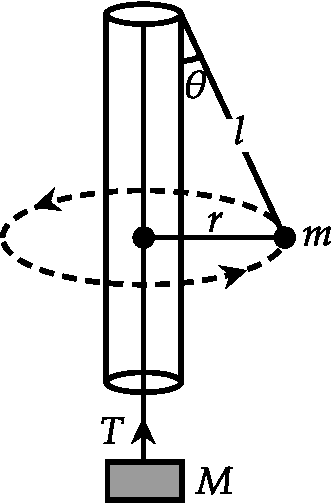
\includegraphics[height=5cm,width=3.5cm]{pq05}
	\end{figure}
	\begin{answer}
		\begin{align*}
		\text{Tension in the string }\mathrm{T}&=\mathrm{Mg}\\
		\text{Centripetal force on the body }&=\operatorname{mr} \omega^{2}=\operatorname{mr}(2 \pi \mathrm{v})^{2}
		\intertext{ This is provided by the component of tension acting horizontally i.e. $T \sin \theta=M g \sin \theta $.}
		\therefore \mathrm{mr}(2 \pi v)^{2}&=\mathrm{} \sin \theta=
		\mathrm{Mg} \frac{r}{l} \\ v&=\frac{1}{2 \pi} \sqrt{\frac{\mathrm{Mg}}{\mathrm{m l} }}
		\end{align*}
	\end{answer}
	\item A string of negligible mass going over a clamped pulley of mass $\mathrm{m}$ supports a block of mass $M$ as shown in fig. The force on the pulley by the clamp is given by\\
	\begin{figure}[H]
		\centering
		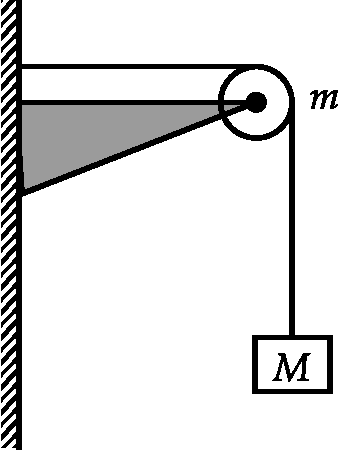
\includegraphics[height=4.5cm,width=3.2cm]{pq06}
	\end{figure}
	\begin{tasks}(2)
		\task[\textbf{A.}]$\sqrt{2} \mathrm{Mg}$
		\task[\textbf{B.}] $\sqrt{2} \mathrm{mg}$
		\task[\textbf{C.}]  $\left[\sqrt{\left.(\mathrm{M}+\mathrm{m})^{2}+\mathrm{m}^{2}\right]} \mathrm{g}\right.$
		\task[\textbf{D.}] $\left[\sqrt{\left.(\mathrm{M}+\mathrm{m})^{2}+\mathrm{M}^{2}\right]} \mathrm{g}\right.$
	\end{tasks}
	\begin{answer}
		\begin{align*}
		\intertext{Force on the pulley by the clamp $=$ resultant of $\mathrm{T}=(\mathrm{M}+\mathrm{m}) \mathrm{g}$ and $\mathrm{mg}$ acting along horizontal and vertical respectively}
		\therefore \mathrm{F}&=\sqrt{[(\mathrm{M}+\mathrm{m}) \mathrm{g}]^{2}+(\mathrm{mg})^{2}}\\&=\left[\sqrt{(\mathrm{M}+\mathrm{m})^{2}+\mathrm{m}^{2}}\right] \mathrm{g}
		\end{align*}
		So the correct answer is \textbf{Option (C)}
	\end{answer}
	\item Find the mass $M$ of the hanging block in figure which will prevent smaller block from slipping over the triangular block. All surfaces are frictionless and the string and the pulley are light.
	\begin{figure}[H]
		\centering
		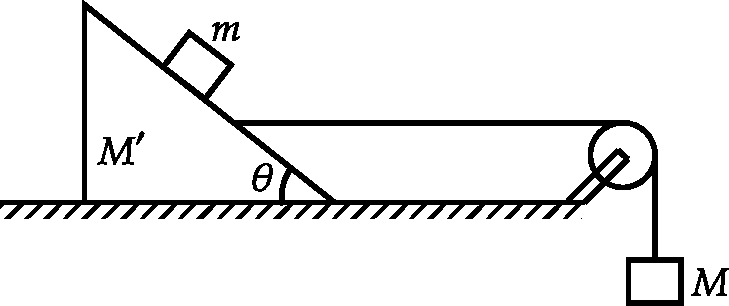
\includegraphics[height=2.7cm,width=6cm]{pq09}
	\end{figure}
	\begin{answer}
		\begin{align}
		\intertext{Since $\mathrm{m}$ does not slip on M' (relative velocity of $\mathrm{m}$ w.r.t. M' is zero)}\notag
		\intertext{$\therefore \mathrm{M}^{\prime}, \mathrm{m}$ will move with same acceleration as that of $\mathrm{M}$, Since surfaces are smooth}\notag
		\text{$\therefore$ frictional force is zero}\notag\\
		\text{Net force }&=\mathrm{Mg}=\left(\mathrm{M}+\mathrm{M}^{\prime}+\mathrm{m}\right) \mathrm{a}\notag\\
		\therefore \mathrm{a}&=\frac{\mathrm{Mg}}{\mathrm{M}+\mathrm{M}^{\prime}+\mathrm{m}}\label{pq01}
		\intertext{Now let us see m, w.r.t. M'}\notag
		\end{align}
		\begin{figure}[H]
			\centering
			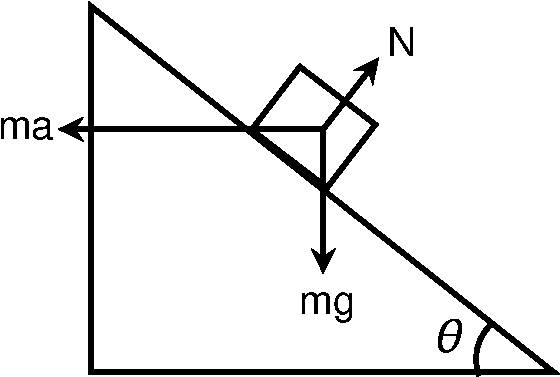
\includegraphics[height=2.5cm,width=4cm]{pq09(2)}
		\end{figure}
		\begin{align}
		\intertext{Downward acceleration of $\mathrm{m}$ on slope $=0$}
		\therefore \mathrm{N}-\mathrm{ma} \sin \theta+\mathrm{mg} \cos \theta&=0\\
		(\text{net }&\perp\text{ force }=0)\notag\\
		\text{and }m g \sin \theta-\operatorname{ma} \cos \theta&=0\label{pq03}\\
		[\because&\text{ net force along slope }=0]\notag\\
		\text{From eq }^{n} \cdot(\ref{pq03}) g \sin \theta=a \cos \theta\text{ or }a&=g \tan \theta\label{pq04}
		\intertext{From eq $^{\mathrm{n}}$. (\ref{pq04}) and (\ref{pq01}),}\notag\\
		\text{we have }\tan \theta&=\frac{M}{M+M^{\prime}+m} \notag\\\Rightarrow M \cot \theta&=M+M^{\prime}+m\notag\\
		\Rightarrow \mathrm{M}&=\frac{\mathrm{M}^{\prime}+\mathrm{m}}{\cot \theta-1}\notag
		\end{align}
	\end{answer}
	\item A mass of $15 kg$ and another of mass $6kg$ are attached to a pulley system as shown in the fig. A is a fixed pulley while $B$ is a movable one. Both are considered light and frictionless. Find the acceleration of $6kg$ mass.
	\begin{figure}[H]
		\centering
		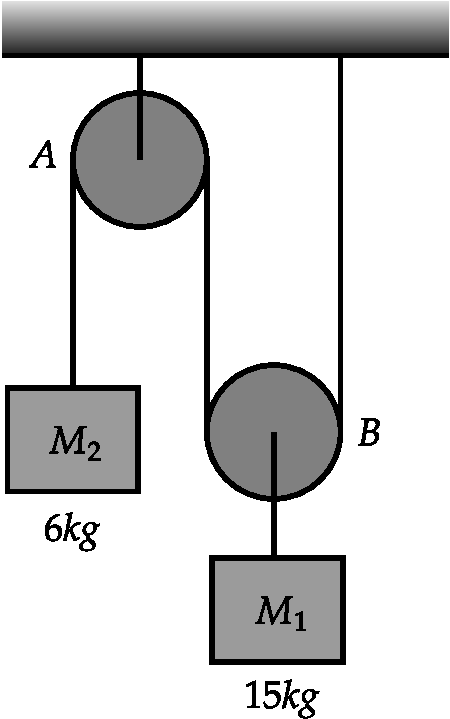
\includegraphics[height=6.5cm,width=4cm]{pq13}
	\end{figure}
	\begin{answer}
		Tension is the same throughout the string. It is clear that $\mathrm{M}_{1}$ will descend downwards while $\mathrm{M}_{2}$ rises up. If the acceleration of $\mathrm{M}_{1}$ is a downwards, $\mathrm{M}_{2}$ will have an acceleration ' $2 \mathrm{a}$ ' upward.
		\begin{figure}[H]
			\centering
			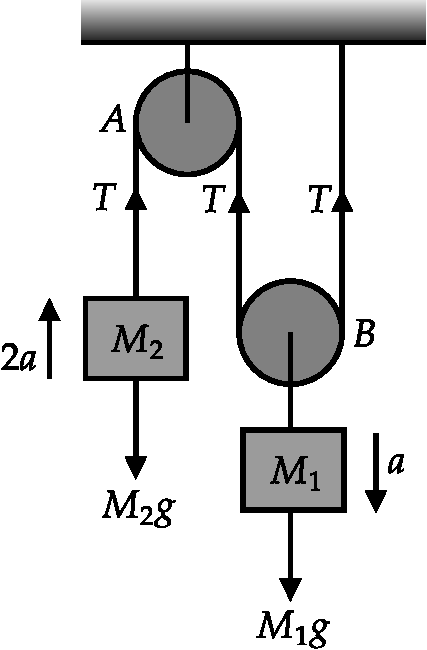
\includegraphics[height=6cm,width=4cm]{pq13(2)}
		\end{figure}
		\begin{align*}
		\intertext{Now,}
		\mathrm{M}_{1} \mathrm{~g}-2 \mathrm{~T}&=\mathrm{M}_{1} \mathrm{a}\\
		\mathrm{T}-\mathrm{M}_{2} \mathrm{~g}&=\mathrm{M}_{2} \cdot 2 \mathrm{a}
		\intertext{or}
		\mathrm{M}_{1} \mathrm{~g}-2 \mathrm{M}_{2} \mathrm{~g}&=\mathrm{a}\left(\mathrm{M}_{1}+4 \mathrm{M}_{2}\right)\\
		\Rightarrow a&=\frac{M_{1}-2 M_{2}}{M_{1}+4 M_{2}} g=\frac{15-12}{15-24} g=\frac{3}{39} g\\
		\therefore \mathrm{a}&=\frac{\mathrm{g}}{13}\\
		\therefore \text{ acceleration of }6 \mathrm{~kg}\text{ mass }&=2 \mathrm{a}=\frac{2 \mathrm{~g}}{13}
		\end{align*}
	\end{answer}
	\item A mass $m$ is revolving in a vertical circle at the end of a string of length $20 \mathrm{~cm}$. By how much does the tension of the string at the lowest point exceed the tension at the topmost point?
	\begin{answer}
		\begin{align*}
		\intertext{The tension $T_{1}$ at the topmost point is given by,}
		\mathrm{T}_{1}=\frac{\mathrm{m} \mathrm{v}_{1}^{2}}{20}-\mathrm{mg}
		\intertext{Centrifugal force acting outward while weight acting downward}
		\text{The tension $T_{2}$ at the lowest point, }T_{2}&=\frac{m v_{2}^{2}}{20}+m g
		\intertext{Centrifugal force and weight (both) acting downward}
		\mathrm{T}_{2}-\mathrm{T}_{1}&=\frac{\mathrm{m} \mathrm{v}_{2}{ }^{2}-\mathrm{m} \mathrm{v}_{1}^{2}}{20}+2 \mathrm{mg} ; \\ \mathrm{v}_{1}^{2}&=\mathrm{v}_{2}^{2}-2 \mathrm{~g} \mathrm{~h}\text{ or}\\
		\mathrm{v}_{2}^{2}-\mathrm{v}_{1}^{2}&=2 \mathrm{~g}(40)=80 \mathrm{~g}\\
		\therefore \quad T_{2}-T_{1}&=\frac{80 \mathrm{mg}}{20}+2 \mathrm{~m} \mathrm{~g}=6 \mathrm{mg}
		\end{align*}
	\end{answer}
	\item 
	A block of mass $m$ is placed on a smooth wedge of inclination $\theta$. The whole system is accelerated horizontally so that the block does not slip on the wedge. The force exerted by the wedge on the block (g is acceleration due to gravity) will be
	\begin{tasks}(4)
		\task[\textbf{A.}]	$\mathrm{mg} / \cos \theta$
		\task[\textbf{B.}] $\mathrm{mg} \sin \theta$
		\task[\textbf{C.}] $m g \cos \theta$
		\task[\textbf{D.}] $\mathrm{mg}$
	\end{tasks}
	\begin{answer}
		\begin{align}
		N&=m a \sin \theta+m g \cos \theta\\
		\text{also }\mathrm{m} \mathrm{g} \sin \theta&=\mathrm{m} \operatorname{a} \cos \theta\label{pq06}\\
		\text{from }(\ref{pq06}) a&=g \tan \theta\notag\\
		\therefore \mathrm{N}&=\mathrm{mg} \frac{\sin ^{2} \theta}{\cos \theta}+\mathrm{mg} \cos \theta\notag\\
		\text{or }N&=\frac{m g}{\cos \theta}\notag
		\end{align}
		\begin{figure}[H]
			\centering
			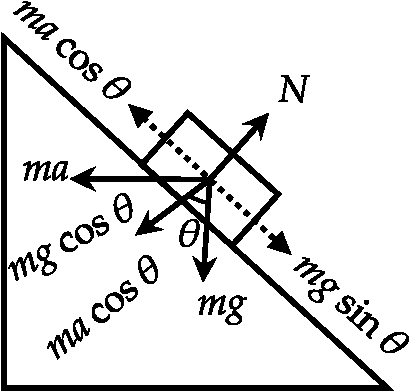
\includegraphics[height=4cm,width=4cm]{pq05(s)}
		\end{figure}
		So the correct answer is \textbf{Option (A)}
	\end{answer}
	\item The coefficient of static friction, $\mu_{\mathrm{s}}$, between block $\mathrm{A}$ of mass $2 \mathrm{~kg}$ and the table as shown in the figure is $0.2$. What would be the maximum mass value of block $\mathrm{B}$ so that the two blocks do not move? The string and the pulley are assumed to be smooth and massless. ( $\left.\mathrm{g}=10 \mathrm{~m} / \mathrm{s}^{2}\right)$
	\begin{figure}[H]
		\centering
		\includegraphics[height=3cm,width=5cm]{pq07}
	\end{figure}
	\begin{tasks}(4)
		\task[\textbf{A.}]$0.4 \mathrm{~kg}$
		\task[\textbf{B.}] $4.0 \mathrm{~kg}$
		\task[\textbf{C.}] $2.0 \mathrm{~kg}$
		\task[\textbf{D.}] $0.2 \mathrm{~kg}$
	\end{tasks}
	\begin{answer}
		\begin{align*}
		\mathrm{m}_{\mathrm{B}} \mathrm{g}&=\mu_{\mathrm{s}} \mathrm{m}_{\mathrm{A}} \mathrm{g} \quad\left\{\because \mathrm{m}_{\mathrm{A}} \mathrm{g}=\mu_{\mathrm{s}} \mathrm{m}_{\mathrm{A}} \mathrm{g}\right\}\\
		\Rightarrow \mathrm{m}_{\mathrm{B}}&=\mu_{\mathrm{s}} \mathrm{m}_{\mathrm{A}}\\
		\text{	or }m_{B}&=0.2 \times 2=0.4 \mathrm{~kg}
		\end{align*}
		So the correct answer is \textbf{Option (A)}
	\end{answer}
	\item A person of mass $60 \mathrm{~kg}$ is inside a lift of mass $940 \mathrm{~kg}$ and presses the button on control panel. The lift starts moving upwards with an acceleration $1.0 \mathrm{~m} / \mathrm{s}^{2}$. If $\mathrm{g}=10 \mathrm{~ms}^{-2}$, the tension in the supporting cable is
	\begin{tasks}(4)
		\task[\textbf{A.}]$8600 \mathrm{~N}$
		\task[\textbf{B.}] $9680 \mathrm{~N}$
		\task[\textbf{C.}] $11000 \mathrm{~N}$
		\task[\textbf{D.}]  $1200 \mathrm{~N}$
	\end{tasks}
	\begin{answer}$\left. \right. $
		\begin{figure}[H]
			\centering
			\includegraphics[height=3cm,width=4cm]{pq06(s)}
		\end{figure}
		\begin{align*}
		\text{	Total mass }&=(60+940) \mathrm{kg}=1000 \mathrm{~kg}
		\intertext{Let $\mathrm{T}$ be the tension in the supporting cable, then}
		\mathrm{T}-1000 \mathrm{~g}&=1000 \times 1\\
		\Rightarrow \mathrm{T}&=1000 \times 11=11000 \mathrm{~N}
		\end{align*}
		So the correct answer is \textbf{Option (C)}
	\end{answer}
	\item A given object takes $\mathrm{n}$ times as much time to slide down a $45^{\circ}$ rough incline as it takes to slide down a perfectly smooth $45^{\circ}$ incline. The coefficient of kinetic friction between the object and incline is given by
	\begin{tasks}(4)
		\task[\textbf{A.}]$\left(1-\frac{1}{n^{2}}\right)$
		\task[\textbf{B.}] $\frac{1}{1-\mathrm{n}^{2}}$
		\task[\textbf{C.}] $\sqrt{\left(1-\frac{1}{n^{2}}\right)}$
		\task[\textbf{D.}] $\sqrt{\left(\frac{1}{1-\mathrm{n}^{2}}\right)}$
	\end{tasks}
	\begin{answer}
		\begin{align*}
		\text{	We have }\sqrt{\frac{2 s}{g(\sin \theta-\mu \cos \theta)}}&=n \sqrt{\frac{2 s}{g \sin \theta}}\\
		\frac{2 s}{g(\sin \theta-\mu \cos \theta)}&=\frac{2 s \times n^{2}}{g \sin \theta}\\
		\text{here }\theta&=45^{\circ} \Rightarrow \frac{1}{1-\mu}=\mathrm{n}^{2}\\ \text{ or } \mu&=\left(1-1 / \mathrm{n}^{2}\right)
		\end{align*}
		So the correct answer is \textbf{Option (A)}
	\end{answer}
	\item Two fixed frictionless inclined planes making an angle $30^{\circ}$ and $60^{\circ}$ with the vertical are shown in the figure. Two blocks A and $B$ are placed on the two planes. What is the relative vertical acceleration of $A$ with respect to $B$ ?
	\begin{figure}[H]
		\centering
		\includegraphics[height=3cm,width=5.5cm]{pq091}
	\end{figure}
	
	\begin{answer}
		\begin{align*}
		m g \sin \theta&=m a\\
		\therefore a&=g \sin \theta\\
		&\text{where a is along the inclined plane}\\
		\therefore&\text{vertical component of acceleration is $g \sin ^{2} \theta$}\\
		\intertext{Then the  relative vertical acceleration of $\mathrm{A}$ with respect to $\mathrm{B}$ is}
		g\left(\sin ^{2} 60-\sin ^{2} 30\right]&=\frac{g}{2}\\&=4.9 \mathrm{~m} / \mathrm{s}^{2}\quad
		(\text{in vertical direction})
		\end{align*}
	\end{answer}
\end{enumerate}
